\documentclass[10pt,a4paper]{article}
\usepackage[utf8]{inputenc}
\usepackage[german]{babel}
\usepackage{amsmath}
\usepackage{amsfonts}
\usepackage{amssymb}
\usepackage{graphicx} %Um Bilder anzeigen zu können
\usepackage[top=1in, bottom=1.5in, left=1in, right=1in]{geometry}

\title{\Huge Pflichtenheft\\[1cm] {\bfseries Praxis der Softwareentwicklung}\\Gruppe 1\\[2cm] Entwicklung einer Software zur Berechnung der Mandatsverteilung im Deutschen\\[1cm] }
\author{Philipp Löwer, Anton Mehlmann, Manuel Olk, Enes Ördek, \\Simon Schürg, Nick Vlasoff}
\date{}

\begin{document}
\maketitle

\begin{figure}[h]

\centering
		
		
\includegraphics[scale=0.6]{KIT-Logo.png}\\
		\Huge WS 2013 / 14
\end{figure}

		
\newpage
\tableofcontents

\section{Produktübersicht}
Bei dem Produkt handelt es sich um ein Programm, das die Sitzverteilung im Deutschen Bundestag gemäß der gesetzlichen Bestimmungen exakt berechnet und deren Zustandekommen verständlich darlegt. Erreicht wird dies durch eine minimalistische und intuitive Benutzeroberfläche.

\subsection{Lizenz}
Der Quellcode des Programms wird der Öffentlichkeit frei zur Verfügung gestellt. Es wird die GPL V3 Lizenz verwendet, damit das Projekt nach einer Modifizierung weiterhin öffentlich bleibt.

\section{Zielbestimmung}
\subsection{Musskriterien}
\begin{itemize}
\item Auswertung von Wahlergebnissen nach gesetzlicher Bestimmung
\item Grafische Benutzeroberfläche
\item Vergleich mehrerer Wahlausgänge
\item Importmöglichkeit von Wahlergebnissen (.csv)
\item Manipulation von Eingabedaten
\end{itemize}

\subsection{Sollkriterien}
\begin{itemize}
\item Auffinden paradoxer Wahlausgänge
\item Kartographische Darstellung der Bundesländer
\end{itemize}

\subsection{Kannkriterien}
\begin{itemize}
\item Hilfe (Benutzerhandbuch)
\end{itemize}


\subsection{Abgrenzungskriterien}
\begin{itemize}
\item Keine Mobile Anwendung oder Web-App
\item Keine namentliche Nennung von Abgeordneten
\end{itemize}


\section{Produkteinsatz}
\subsection{Anwendungsbereiche}
\begin{itemize}
\item Überprüfung der Wahlergebnisse
\end{itemize}


\subsection{Zielgruppen}
\begin{itemize}
\item Menschen, die kritisch gegenüber Wahlergebnissen sind
\item (Unabhängige) Medien
\item Politisch Interessierte
\end{itemize}


\subsection{Betriebsbedingungen}
\begin{itemize}
\item Keine Verbindung zum Internet nötig
\end{itemize}


\section{Produktumgebung}
\subsection{Software}
\begin{itemize}
\item Java Runtime Environment SE 1.7 oder neuer.
\item Betriebssystem z.B. Windows, Linux, Mac OS
\end{itemize}


\subsection{Hardware}
Mindestanforderungen:
\begin{itemize}
\item Bildschirmauflösung: 1024x768
\end{itemize}


\subsection{Orgware}
\begin{itemize}
\item Keine weiteren Rahmenbedingungen notwendig
\end{itemize}


\subsection{Schnittstellen}
\begin{itemize}
\item Importieren/ Exportieren von Zuständen und Daten
\end{itemize}


\section{Funktionale Anforderungen}
Funktionale Anforderungen werden durch eine vierstellige Nummer gekennzeichnet. Die erste Nummer kennzeichnet den folgenden Bereich:
\begin{itemize}
	\item GUI (View)
	\item Schnittstellen (Controller)
	\item Datenhaltung (Model)
\end{itemize}
Die restlichen Nummern dienen zur Durchnummerierung.

\subsection{GUI (View)}
\begin{itemize}
	\item /F10010/ Programmstart \hfill \\
	Initialisierung des Hauptfensters. Es wird, falls vorhanden, der letzte Programmzustand aufgerufen (/F20010/). Andernfalls lädt das Programm die Daten der letzten Bundestagswahl.
	\item /F10020/ Menü \hfill \\
	Im Menü sind folgende Punkte gelistet:
	\begin{itemize}
		\item Datei
		\begin{itemize}
			\item Speichern des aktuellen Zustandes /F20010/
			\item Laden eines Zustandes /F20011/
			\item Importieren von Daten /F20020/
			\item Exportieren von Daten /F20030/
		\end{itemize}
		\item Bearbeiten
		\begin{itemize}
			\item Rückgängig /F20040/
		\end{itemize}
		\item Extras
		\item Hilfe /F10030/
	\end{itemize}
	\item /F10030/ Hilfe \hfill \\
	Durch den Klick auf diesen Menüpunkt öffnet sich ein Fenster, in der Handbücher zum Programm zu finden sind. Des weiteren ein kleines About, mit den wichtigsten Informationen zum Programm.
	\item /F10050/ Kartografische Darstellung der Länder \hfill \\
	Die Länder werden nach einer überprüfung (/F30010/), Kartografisch im Fenster dargestellt.
	\item /F10100/ Programmende \hfill \\
	Das Programm speichert den aktuellen Zustand (/F20010/) und schließt das Programm.
\end{itemize}

\subsection{Schnittstellen (Controller)}
\begin{itemize}
	\item /F20010/ Speichern des aktuellen Programmzustandes \hfill \\
	Es wird das Zustands-Objekt (/PD01/) in einer Datei abgelegt. Dabei kann der Benutzer beim Speichern einen internen Namen und ein Kommentar abgeben, welche mit gespeichert werden.
	\item /F20011/ Laden eines Programmzustandes \hfill \\
	Der Benutzer wählt eine Datei aus. Es wird überprüft, ob es sich um ein gültiges Objekt handelt. Falls die Version unterschiedlich ist, wird die Datei konvertiert und geladen.
	\item /F20020/ Importieren von Daten \hfill \\
	Die .csv-Dateien des Bundeswahlleiters können importiert werden.
	\item /F20025/ Filtern der relevanten Daten \hfill \\
	Die benötigten Dateien werden aus der ausgewählten .csv-Datei geladen und zu der Model-Klasse geschickt.
	\item /F20030/ Exportieren von Daten \hfill \\
	Daten können als .csv-Dateien oder als JSON/XML exportiert werden.
	\item /F20040/ Rückgängig machen \hfill \\
	Es können Operationen rückgängig gemacht werden. Hierfür wird das History-Objekt (/PD05/) verwendet.
\end{itemize}

\subsection{Datenhaltung und Verarbeitung (Model)}
\begin{itemize}
	\item /F30010/ Überprüfen der Ländernamen \hfill \\
	Überprüft ob die eingegebenen Ländernamen in dem Daten-Objekt (/PD03/) korrekt sind. Falls alle Ländernamen gefunden werden, wir die Kartografische Darstellung (/F10050/) aktiviert.
	\item /F30020/ Überprüfen der Stimmen\hfill \\
	Überprüft ob die eingegebenen Stimmen in dem Daten-Objekt (/PD03/) korrekt sind. Falls die Anzahl der Stimmen $\geq$ 0 sind, kann die Sitzverteilung mit dem Wahlgesetz-Objekt (/PD04/) berechnet werden.
\end{itemize}
\section{Produktdaten}
\begin{itemize}
	\item /PD01/ Zustands-Object \hfill \\
	Repräsentiert den aktuellen Zustand des Programms. Es beinhaltet alle Informationen, um den genauen Zustand des Programms wiederherzustellen. Es handelt sich um eine serialisierbare Klasse.
	\begin{itemize}
		\item Version des Programms (um Abwärtskompatibilität zu gewährleisten)
		\item Datum und Uhrzeit der Erstellung
		\item Name/ID
		\item Kommentar
		\item Fenster-Objekt als Liste
		\item History-Objekt
	\end{itemize}
	
	\item /PD02/ Fenster-Objekt
	\begin{itemize}
		\item Wahlergebnisse (Daten-Objekt)
		\item Wahlgesetz-Objekt
		\item Name/ID
	\end{itemize}
	
	\item /PD03/ Daten-Objekt \hfill \\
	Beinhaltet die Anzahl der (Erst- und Zweit-)Stimmen je Wahlkreis und Partei.
	\begin{itemize}
		\item Name/ID
		\item Kommentar (Quelle)
		\item Wahlkreise mit Stimmen als Array.
	\end{itemize}
	
	\item /PD04/ Wahlgesetz-Objekt \hfill \\
	Beinhaltet das Algorithmus zur Berechnung der Sitze mit dem Daten-Objekt als Eingabedatum.\\
	Des weiteren überprüft das Objekt, ob mit dem Datenobjekt eine Wahl überhaupt simuliert werden kann (wenn ein Datenobjekt beispielsweise keine Erststimmen enthält wie in sehr alten Wahlen).
	
	\item /PD05/ History-Objekt \hfill \\
	Dieses Objekt zeichnet alle Veränderungen am Programm auf. Mithilfe dieses Objektes können Operationen über das Menü Bearbeiten oder STRG+Z rückgängig gemacht werden (/F10020/ und /F20040/).
\end{itemize}
\section{Produktleistungen}
\begin{itemize}
	\item Zeit
	\begin{itemize}
		\item Starten + Laden des letzten Zustandes: unter 5 Sekunden.
		\item Beenden + Speichern des aktuellen Zustandes: unter 5 Sekunden.
		\item Exportieren/Importieren von Daten: unter 10 Sekunden.
	\end{itemize}
	\item Genauigkeit \hfill \\
	Die Genauigkeit des Algorithmus zur Sitzberechnung muss dem Wahlgesetz entsprechen und exakte Ergebnisse liefern.
\end{itemize}
\section{Nicht-funktionale Anforderungen}
\begin{itemize}
	\item Allgemeine Anforderungen:
	\begin{itemize}
		\item Die Sitzverteilung muss für den Benutzer transparent und nachvollziehbar dargestellt werden.
	\end{itemize}
	\item Sicherheitsanforderungen:
	\begin{itemize}
		\item Die Eingabedaten dürfen während der Berechnung nicht verändert werden.
	\end{itemize}
	\item Plattformunabhängigkeit: \hfill \\
	Das Programm muss auf der offiziellen Oracle JRE laufen.
\end{itemize}
\section{Qualitätsanforderungen}
\begin{itemize}
	\item Hilfreiche Fehlermeldungen
	\item Kein Datenverlust (auch nach Programmabstürzen)
\end{itemize}
\newpage
\section{Globale Testfälle und Szenarien}
Folgende Funktionssequenzen sind zu überprüfen:

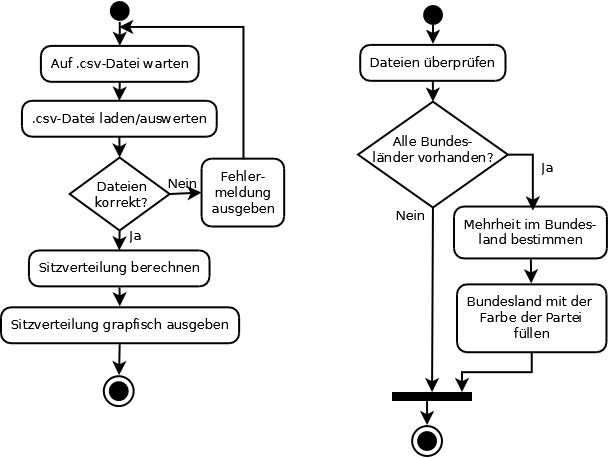
\includegraphics[scale=0.4]{Diagramm1} \\
Folgende Datenkonsistenzen müssen eingehalten werden:
\begin{itemize}
	\item noch nichts...
\end{itemize}
Folgende unzulässige Aktionen müssen korrekt behandelt werden:
\begin{itemize}
	\item Negative Stimmenanzahl
	\item Buchstaben als Stimmen
\end{itemize}
Testszenarien:
\begin{itemize}
	\item Falsche Daten importieren: \newline
	Starten des Programms $\rightarrow$ Im Hauptmenü auf Datei klicken $\rightarrow$ Datei importieren auswählen $\rightarrow$ Im Dateibrowser die falsche .csv-Datei auswählen $\rightarrow$ Mit dem Button Laden bestätigen $\rightarrow$ Eine Fehlermeldung taucht auf $\rightarrow$ Programm befindet sich wieder im Startzustand
	\item Manuell Daten modifizieren: \\
	Starten des Programms $\rightarrow$ Korrekte Daten laden $\rightarrow$ Die Sitzverteilung wird angezeigt $\rightarrow$ Den Wert zweier Parteien miteinander tauschen $\rightarrow$ Die Sitzverteilung erneut berechnen $\rightarrow$ Eine mögliche Veränderung der Sitzverteilung wird angezeigt
	
\end{itemize}
\section{Systemmodelle}
\subsection{Systemarchitektur}
Das Programm basiert auf der MVC- Architektur, wobei auf eine saubere Trennung der Einheiten Model, View und Controller geachtet wird. Dies sorgt nicht nur für einen flexiblen Programmentwurf, so dass spätere Änderungen bzw. Erweiterungen erleichtert werden, sondern garantiert auch die Trennung kritischer Komponenten, wie der Algorithmusimplementierung, von weniger sensiblen Komponenten, wie der GUI, und dient allgemein der Übersichtlichkeit.

\section{Benutzungsoberfläche}

\section{Spezielle Anforderungen an die Entwicklungsumgebung}
\begin{itemize}
	\item Allgemein
	\begin{itemize}
		\item Latex
		\item Versionskontrolle mit SVN
	\end{itemize}
	\item Entwicklung
	\begin{itemize}
		\item IDE: Eclipse
	\end{itemize}
	\item Entwurf
	\begin{itemize}
		\item DIA für Diagramme
	\end{itemize}
	\item Validierung
	\begin{itemize}
		\item JUnit
	\end{itemize}
	\item Teamkommunikation
	\begin{itemize}
		\item Google-Groups Mailingliste
	\end{itemize}
\end{itemize}

\section{Zeit- und Ressourcenplanung}

\section{Ergänzungen}

\section{Glossar}



\end{document}
